% Case Description: Smartly HLK
% deployment setup diagram
\begin{figure*}[b]
\centering
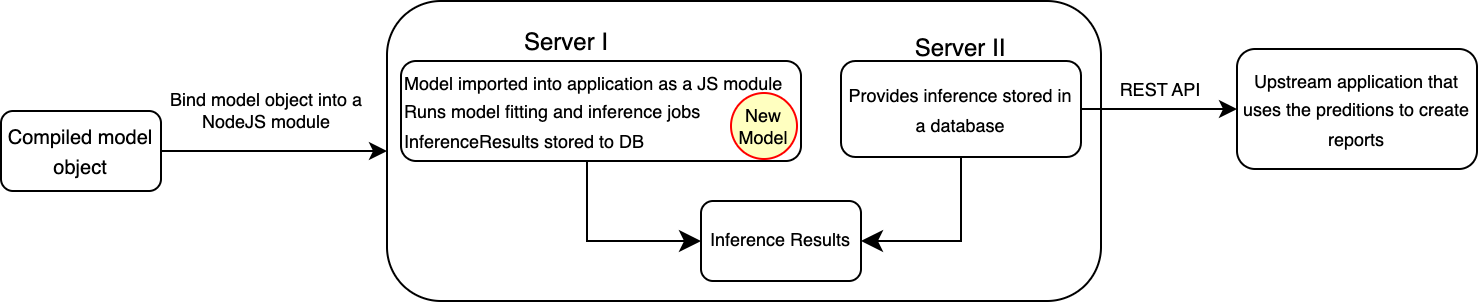
\includegraphics[width=\linewidth]{images/case1_deployment_process.png}
\caption{Case 1 Inference Architecture}
\label{fig: case1_deployment_process}
\end{figure*}

The ML system is part of an advertisement budget allocation system in marketing campaigns. The system uses data from a browsing session context to determine the probability of an Advert viewer converting into a purchaser. The model is built by specifying a STAN\footnote{https //mc-stan.org} program using the STAN\footnote{Stan is a C++ library for Bayesian modelling and Inference that primarily uses the No-U-Turn sampler (NUTS) (Hoffman and Gelman 2012) to obtain posterior simulations given a user-specified model and data.} modelling language. This model differs from typical ML frameworks with distinct fitting/training and inference phases. The model's estimation and Inference occur concurrently in the STAN framework runtime.

\textit{Pre-Integration}: Since no estimated weights and parameters are optimized, a Bayesian model description is compiled into a binary object. The model binary object is packaged as a NodeJS library by binding the model into a nodeJS module. This allows the model to be imported into other Java applications. Updating the model in this setup begins with generating a new version of the code file and re-compiling the file into a new binary object. The business case requires that the model is fitted and new predictions generated daily since consumer behaviour can change drastically, and the Ads should remain highly relevant. To put the scale of operations into perspective, one client can have multiple marketing campaigns, resulting in hundreds of models being updated and used to generate Inference daily.

\textit{Quality assurance}: Quality management is based on performing local tests on the resulting accuracy of the models. These tests are conducted locally and manually orchestrated. The large number of models brings along challenges in identifying faulty models.
% Challenge due to the operations' scale and re-training frequency (Find audio segment reference). This can form part of the discussion topics.

\textit{Server environment}: The deployment setup involves two types of servers: server type I and server type II. Server type I is dedicated to model fitting, generating predictions using the nodes module, and storing the forecasts in a central results database. Server type II is dedicated to serving the prediction results by fetching them from the results database using a REST API. A depiction of this setup is shown in Figure~\ref{fig: case1_deployment_process}. This second server presents the budget allocation service. Batch results are analyzed from this second server daily, and the underlying infrastructure is based on 25 computing nodes. These nodes are separated into a group that performs modelling and inference workloads, while another group is dedicated to providing the inference service API endpoints.

\textit{Inference}: The inference service supports batch and real-time Inference using a REST API that uses JSON to serialize the input and output data. Results from batch inference are stored in an internal data lake accessed by the web server supporting a REST API.

\textit{Monitoring}: Conducted to monitor model accuracy errors and service level errors. Model accuracy is checked through local quick checks, such as the standard deviation of predictions. Due to many models, service level errors are monitored closely because they tend to indicate more significant problems in the system.

% resizing or dedicated page presentation


